%---------------------------------------------------------------
\chapter{Related work}
%---------------------------------------------------------------
\label{ch:related_work}

The process of downscaling -- enhancing image resolution -- has been extensively studied.
The approaches employed fall into two broad categories -- task-independent and task-specific downscaling.
Task-independent downscaling focuses on increasing the resolution of images without explicit context.
Commonly used datasets (e.g. in~\cite{Harder2023, Lim2017, Abrahamyan2022}) to train and evaluate methods, such as Urban100~\cite{Huang2015} and DIV2K~\cite{Timofte2017}, include urban photos, portraits, and pictures of nature and animals.
On the other hand, task-specific downscaling is restricted only to a small subset of images.
Oriani et al.~\cite{Oriani2021} performed task-specific downscaling of satellite images.
However, in this work we will focus specifically on climate data downscaling.
As climate data sources are usually chosen ERA5~\cite{Harder2023, Yang2024, Prasad2024, Perez2024, Sinha2025, Rocha2025}, NorESM~\cite{Harder2023, Prasad2024}, EURO-CORDEX~\cite{Jacob2014, Kostal2025}, ECMWF~\cite{Price2022}, and ReKIS\footnote{\url{https://rekisviewer.hydro.tu-dresden.de/viewer/rekis_domain/KlimRefDS_v3.1_1961-2023.html}}~\cite{Kostal2025, Quesada2023}.

\section{Neural network}

In recent studies, mostly neural networks are employed in downscaling~\cite{Prasad2024, Kostal2025}.
Therefore, in this section, only a brief introduction will be covered; more details can be found in Goodfellow et al.~\cite{Goodfellow2016}.

\subsection{Neural network layers}

Neural networks are composed of layers.
Suppose we have $n$ such layers marked $f^{(i)} \colon \mathbb{R}^{m_i} \to \mathbb{R}^{m_i + 1}$, where $m_i$ is the dimension of the input of $i$-th layer and $m_{i + 1}$ is both the dimension of the output of the $i$-th layer and the dimension of the input of the $(i + 1)$-th.
Therefore, the neural network can be defined by these layers, as shown in Equation~\eqref{e:neural_network}.

\begin{equation}
    \mathbf{f} \coloneqq f^{(n)} \circ f^{(n-1)} \circ \dots \circ f^{(2)} \circ f^{(1)}
    \label{e:neural_network}
\end{equation}

The sole requirement for a function $f^{(i)}$ to be a neural network layer is that it is differentiable \textit{almost everywhere} with respect to each of its inputs.
In the following subsections, we present some of the most common ones and those used in this work.

\subsubsection{Linear layer}

The most common network layer is the linear (sometimes referred to as a dense) neural network layer. 
If we denote the layer as $f \colon \mathbb{R}^{n_{\text{in}}} \to \mathbb{R}^{n_{\text{out}}}$ and $f(x)$ being $f(x) = (f_1(x), \dots, f_{n_\text{out}}(x))$, the linear neural network layer has these $f_i$ functions in the form of:
\begin{equation}
    f_i(x) = w_i^Tx + b_i,
\end{equation}
where $w_i\in \mathbb{R}^{n_\text{in}}$ are the learnable weights and $b_i \in \mathbb{R}$ is the learnable bias.

\subsubsection{Convolutional layer}

The convolution setup regarding machine learning is described by Goodfellow et al.~\cite{Goodfellow2016}.
The operation of convolution has its roots in physical signal processing.
Its main goal is to smooth out the noisy signal; how the smoothing is exactly done is controlled by the choice of kernel.
Convolution is usually denoted by an asterisk, and its formal definition is as follows:
\begin{equation}
    (x \star w)(t) = \int x(a)s(t-a) \mathrm{d}a .
\end{equation}
This relation can be straightforwardly converted to the multidimensional case.
Then its two-dimensional discrete form is:
\begin{equation}
    (I \star K)_{i,j} = \sum_m\sum_nI(m, n)K(i-m, j-n).
\end{equation}
However, this version is not implemented in machine learning libraries, e.g. PyTorch~\cite{PyTorchConv2d}.
Instead of true convolution, what is actually used is cross-correlation, as defined in Equation~\eqref{e:cross_correlation} and visualized in Figure~\ref{fig:convolution}.
The change is equivalent to flipping the kernel.

\begin{equation}
    (K \star I)_{i,j} = \sum_m\sum_nI(i+m, j+n)K(m, n).
\label{e:cross_correlation}
\end{equation}

\begin{figure}
    \centering
    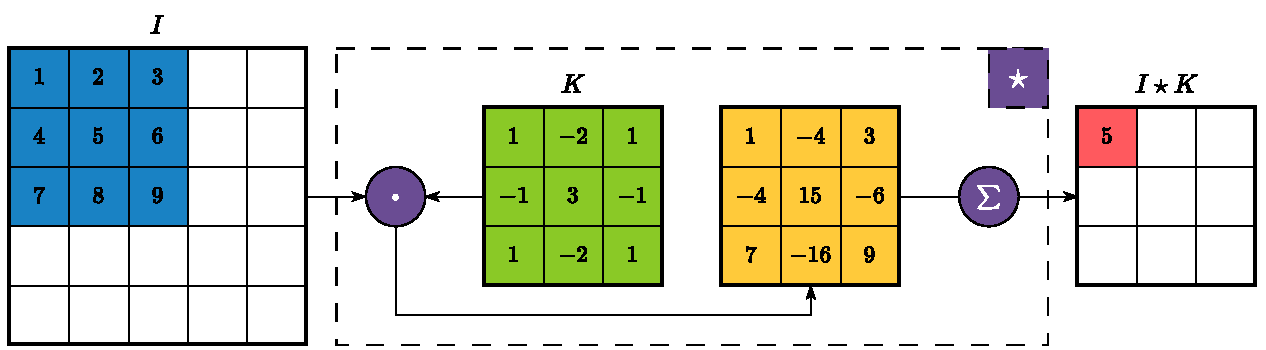
\includegraphics[width=\linewidth]{images/convolution.pdf}
    \caption[Convolution]{Convolution. Visualization of Equation~\eqref{e:cross_correlation}.}
    \label{fig:convolution}
\end{figure}
\newpage
In image processing, a convolution operation can involve more parameters than just the kernel itself. 
In this work, we will frequently refer to the following three:
\begin{description}
    \item[Stride.]
    Convolution operates by moving the kernel over the image.
    The size of each movement is called the stride.
    In PyTorch~\cite{PyTorchConv2d}, the default stride is 1.
    A commonly used choice is to set the stride equal to the kernel size.
    In this case, the kernel does not overlap between steps, and with a suitable kernel, this setup can be used to implement an average pooling layer (Section~\ref{sss:pooling}).
    In Figure~\ref{fig:dilate}, convolution with a stride set to 2 is shown.

    \begin{figure}
        \centering
        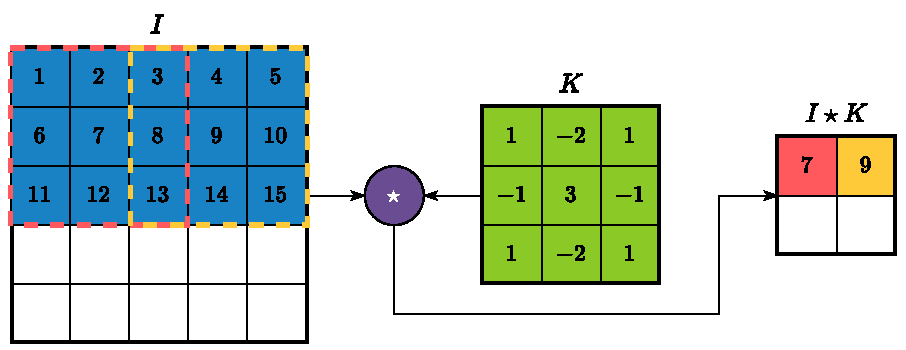
\includegraphics[width=0.75\linewidth]{images/stride.pdf}
        \caption[Stride]{Convolution with stride parameter 2.}
        \label{fig:stride}
    \end{figure}
    
    \item[Dilation.]
    In standard convolution, the kernel is applied to directly adjacent pixels in the image.
    This behavior can be altered by introducing the dilation parameter so that the kernel elements correspond to image pixels that are spaced apart rather than immediately neighboring.
    For a dilation parameter $d$, this is equivalent to convolving with a modified kernel $K'$, constructed by inserting $d-1$ zeros between consecutive values of $K$, as shown in Equation~\eqref{e:dilation}.
    In Figure~\ref{fig:dilate}, convolution with a dilation set to 2 is shown.

\NiceMatrixOptions{xdots/horizontal-labels}
\begin{equation}
    K'=
    \begin{bNiceArray}{ccccccccc}[first-row,last-col,margin]
        & \Hbrace{3}{d-1} \\
        K_{1,1} & 0 & \cdots & 0 & K_{1,2}  & 0 & \cdots & 0 & K_{1, n} \\
        0       &   &        &   &   0      &   &        &   & 0 & \Vbrace{3}{d-1} \\ 
        \vdots  &   & \ddots &   & \vdots   &   & \ddots &   & \vdots \\ 
        0       &   &        &   &   0      &   &        &   & 0 \\
        K_{2,1} & 0 & \cdots & 0 & K_{2,2}  & 0 & \cdots & 0 & K_{2, n} \\
        0       &   &        &   &   0      &   &        &   & 0 \\ 
        \vdots  &   & \ddots &   & \vdots   &   & \ddots &   & \vdots \\ 
        0       &   &        &   &   0      &   &        &   & 0 \\
        K_{m,1} & 0 & \cdots & 0 & K_{m,2}  & 0 & \cdots & 0 & K_{m, n} \\
    \end{bNiceArray}
    \label{e:dilation}
\end{equation}

\begin{figure}
    \centering
    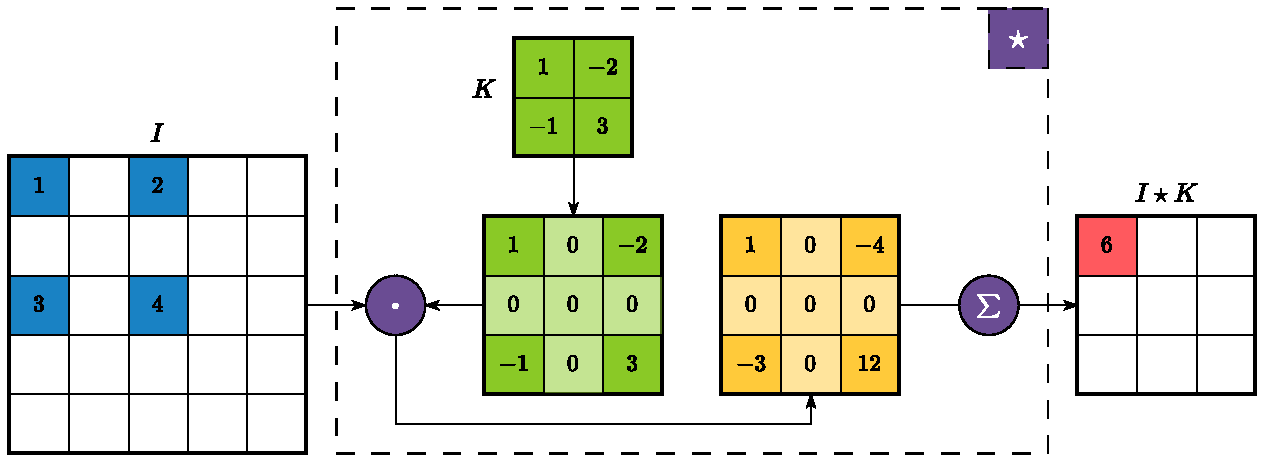
\includegraphics[width=\linewidth]{images/dilate.pdf}
    \caption[Dilation]{Convolution with dilation parameter 2.}
    \label{fig:dilate}
\end{figure}
    
    \item[Padding.]
    A standard convolution applied to an image of dimensions $n_1 \times n_2$ with a kernel of dimensions $k_1 \times k_2$ produces an output image of size $(n_1 - k_1 + 1) \times (n_2 - k_2 + 1)$.
    Thus, by default, the convolution operation decreases the spatial size of the input image.  
    To address this, padding is used.  
    Padding means adding extra rows and columns around the borders of the input image.  
    These added entries can be set to zero, copy the edge values, or even mirror the image content.
    The convolution is then performed on this padded image, and the resulting output can preserve the initial dimensions or even yield a larger image, though the latter is not commonly done.
    
\end{description}

\subsubsection{Pooling layers}
\label{sss:pooling}

Pooling layers closely resemble convolutional layers. 
They share the same core idea of moving a small window -- similar to a kernel -- across the image.
On the other hand, the difference is that these layers do not contain any learnable parameters, and the window usually moves with non-overlapping steps (stride of the window size).

Min-, max-, and average-pooling layers are types of pooling layers where, at each step, the minimum, maximum, or mean value within the window of the image is passed to the output image, respectively.
Furthermore, an average pooling layer with parameter $k$ can be interpreted as a convolution operation with a fixed (non-trainable) $k \times k$ kernel whose entries are all $k^{-2}$, applied with stride $k$.


\subsubsection{Activation function}

A common part of neural networks is the activation functions.
The most widely used activation function is ReLU (Equation~\eqref{e:relu}); however, other alternatives also exist (e.g. LeakyReLU Equation~\eqref{e:leaky_relu}).
These layers do not contain any trainable parameters.

\begin{align}
    \text{ReLU}(x) &\coloneqq \max(0, x) \label{e:relu} \\
    \text{LeakyReLU}(x) &\coloneqq 
        \begin{cases}
            0.01 x & x < 0 \\
            x & x \ge 0
        \end{cases}
        \label{e:leaky_relu}
\end{align}

\subsubsection{Pixel shuffle layer}

In order to perform downscaling, it is necessary to include a layer that increases the spatial resolution. 
One such layer is the pixel shuffle layer~\cite{Shi2016}, which transforms an input image with $C \cdot r^2$ channels and spatial size $H \times W$ into an output with $C$ channels and spatial dimensions $(H \cdot r) \times (W \cdot r)$ by rearranging the feature maps in the way that is illustrated in Figure~\ref{fig:pixel_shuffle}.
This layer has no trainable parameters, and both the values in the feature maps and the number of stored values remain unchanged.
The reverse operation, which takes $C$ channels of spatial size $(H \cdot r) \times (W \cdot r)$ and produces $C \cdot r^2$ channels of spatial size $H \times W$, is referred to as the \textit{pixel unshuffle layer}.

\begin{figure}
    \centering
    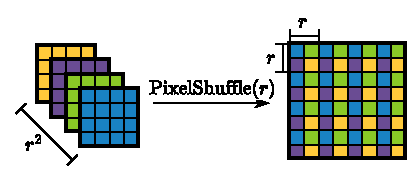
\includegraphics[width=0.5\linewidth]{images/pixel_shuffle.pdf}
    \caption[Pixel shuffle layer]{Pixel shuffle layer. Source: redesigned~\cite{Shi2016}.}
    \label{fig:pixel_shuffle}
\end{figure}
\newpage
\subsection{Evaluation metrics}

An essential part of machine learning is quantifying a model's performance.
Suppose we have a regression task. 
Let $\hat{Y} \in \mathbb{R}^{m, n}$ be the model output -- an image of dimension $m \times n$, and $Y \in \mathbb{R}^{m, n}$ be the target of the same dimension.
Evaluation metrics, therefore, express the difference between the target $Y$ and the model output $\hat{Y}$. 
There are endless possibilities to compare these two matrices; however, only a few are frequently used, such as Mean Square Error (MSE, Equation~\eqref{e:mse}), Mean Absolute Error (MAE, Equation~\eqref{e:mae}), and Root Mean Square Error (RMSE, Equation~\eqref{e:rmse}).
When the objects $Y$ and $\hat{Y}$ are images, these metrics are often referred to as pixel-wise evaluation metrics.

% Tu nie je \begin{equation}, je to problem??
\begin{align}
    \text{MSE}\left(Y, \hat{Y}\right) &\coloneqq \frac{1}{mn} \sum_{i=1}^m \sum_{j=1}^n \left( \hat{Y}_{i,j} - Y_{i,j} \right)^2 \label{e:mse} \\
    \text{MAE}\left(Y, \hat{Y}\right) &\coloneqq \frac{1}{mn} \sum_{i=1}^m \sum_{j=1}^n \left| \hat{Y}_{i,j} - Y_{i,j} \right| \label{e:mae} \\
    \text{RMSE}\left(Y, \hat{Y}\right) &\coloneqq \sqrt{\text{MSE}\left(Y, \hat{Y}\right)} \label{e:rmse}
\end{align}

\subsection{Optimizer}

The optimizer governs how a neural network is trained.
It determines how the model’s weights are updated and how it responds to improvements or declines in performance.
After each step, the gradient of the loss function is computed, and the optimizer uses this information to modify the weights of the layers.
This gradient exists because the loss function and the layers are differentiable.
There exist several algorithms suitable for this setting; however, throughout this work we will employ \textit{Adam}, whose detailed description can be found in~\cite{Kingma2017}.

\subsection{EDSR}

Various architectures are used for the purpose of downscaling in~\cite{Yang2024, Kostal2025, Vandal2017, Groenke2020, Rampal2025}, including Super-Resolution Convolutional Neural Network (SRCNN)~\cite{Dong2015}, Enhanced Deep Super-Resolution Network (EDSR)~\cite{Lim2017}, Normalizing Flows~\cite{Rezende2015}, Fourier Neural Operator (FNO)~\cite{Li2021}, Generative Adversarial Network (GAN)~\cite{Goodfellow2016}, and SwinIR~\cite{Liang2021}.

We will use the same architecture as Košťál et al.~\cite{Kostal2025}, where the EDSR model had a negligible performance difference from the best SwinIR model, although it is a simpler model.
In line with Lim et al.~\cite{Lim2017}, we use the L1 loss (MAE, Equation~\eqref{e:mae}) as the pixel-wise loss function throughout this work, instead of the L2 loss (MSE, Equation~\eqref{e:mse}), since it ``provides better convergence''.

EDSR is a neural network architecture designed by Lim et al.~\cite{Lim2017} specifically for SISR tasks.
Two main parameters influencing the size -- the number of parameters -- of EDSR are the number of residual blocks (\textit{res\_blocks}) and the number of channels (\textit{n\_features}) used within the model.
The whole architecture (Figure~\ref{fig:edsr}) can be divided into head, body, and tail parts.

The head consists of a convolutional layer, which takes the same number of channels as the input channel has and outputs \textit{n\_features} channels.
It is followed by the body, which is made of \textit{res\_blocks} residual blocks and one additional convolutional layer.
EDSR's residual blocks (Figure~\ref{sf:res_block}) were created by removing the batch normalization layers from ResNet's residual blocks~\cite{Lim2017}.
Therefore, EDSR has residual blocks containing two convolutional layers and a ReLU layer in between them; moreover, the residue is scaled by $0.1$ to stabilize the learning process~\cite{Lim2017}.
The body is connected to the head in a residual connection manner (Figure~\ref{sf:edsr}).
Finally, the tail involves an upsampler and a final convolutional layer, which yields the downscaled image with the same number of channels as the input.
The upsampler (Figure~\ref{sf:upsampler}) is made of pairs of convolutional and pixel shuffle layers for each prime factor of the scale factor.
The role of the convolutional layer is to produce $p_i^2 \cdot \textit{n\_features}$ channels, so that after applying the pixel shuffle layer with parameter $p_i$, the number of channels is returned to \textit{n\_features}.

\begin{figure}[h]
    \begin{subfigure}{0.25\linewidth}
        \centering
        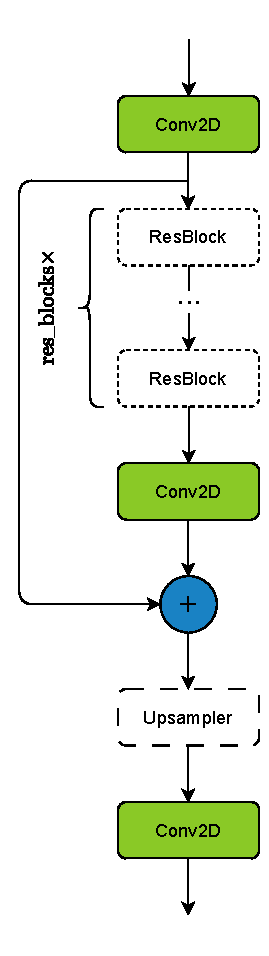
\includegraphics[width=\linewidth]{images/edsr.pdf}
        \caption{EDSR model}
        \label{sf:edsr}
    \end{subfigure}
    \begin{subfigure}{0.22\linewidth}
        \centering
        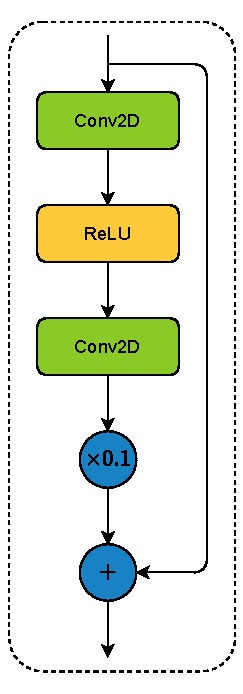
\includegraphics[width=\linewidth]{images/res_block.pdf}
        \caption{Residual block}
        \label{sf:res_block}
    \end{subfigure}
    \begin{subfigure}{0.48\linewidth}
        \centering
        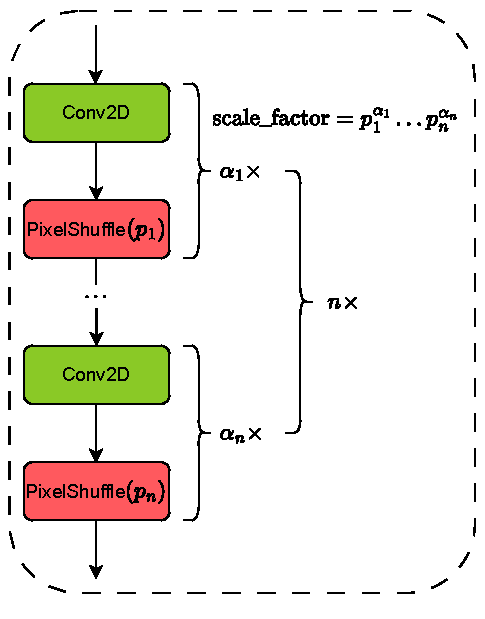
\includegraphics[width=\linewidth]{images/upsampler.pdf}
        \caption{Upsampler}
        \label{sf:upsampler}
    \end{subfigure}
    \caption[EDSR model architecture]{EDSR model architecture with detailed residual block and upsampler architectures. Note that in upsampler, the equation represents the factorization of scale\_factor, therefore $p_i$ are prime numbers. Source: redesigned visualization from Lim et al.~\cite{Lim2017}.}
    \label{fig:edsr}
\end{figure}

\section{Image processing}

Throughout this study, we will treat the climate variables as images, following a SISR-based approach.
Thus, image processing is a fundamental part of this approach used for downscaling; however, since it being a wide field of study, we will include only the necessary techniques used in this work.

We will use the definition of an image by Petrou M. M. P. and Petrou C.~\cite{Petrou2010}.
First, we will define the two-dimensional image function as $f:\mathbb{R} \times \mathbb{R} \to \mathbb{R}$.
The formula of the image function is usually unknown.
Therefore, as an image, we consider a grid sampling of the image function $f$, a real matrix $I \in \mathbb{R}^{m,n}$ having elements $I_{i,j} = f(i,j),\ i \in \{1, 2, \dots m\},\ j \in \{1, 2, \dots n\}$, usually referred to as pixels.

\subsection{Image derivative and gradient}

In this section, we introduced the image function, so it is natural to now discuss its derivatives.
As the image function has a two-dimensional domain, partial derivatives with respect to $x$ (horizontal) and $y$ (vertical) are considered.
Analogous to the image function, the formulas of $\frac{\partial}{\partial x}f$ and $\frac{\partial}{\partial y}f$ are not known in explicit form.
However, the sampled grid is known, and that allows us to make estimates for both partial derivatives.
A straightforward estimate of $\frac{\partial}{\partial x}f$, resp. $\frac{\partial}{\partial y}f$ are differences between neighboring pixels in columns, resp. rows:
\begin{equation}
\begin{aligned}
    \frac{\partial}{\partial x}f(i,j) &\approx I(i,j) - I(i,j+1), \\
    \frac{\partial}{\partial y}f(i,j) &\approx I(i,j) - I(i+1,j)
\end{aligned}
\label{e:simple_derivatives}
\end{equation}
These partial derivatives are also images of dimensions similar to $I$, except for one row and one column, respectively.
The Equations~\eqref{e:simple_derivatives} are implemented as convolutions of image $I$ with the following kernels:
\begin{equation}
K_x = \begin{bmatrix}1 & -1\end{bmatrix}, \qquad K_y = \begin{bmatrix}1 \\ -1\end{bmatrix}.
\label{e:simple_derivative_kernels}
\end{equation}
Therefore, the estimate is made by:
\begin{equation}
    \frac{\partial}{\partial x}f \approx K_x \star I, \qquad
    \frac{\partial}{\partial y}f \approx K_y \star I.
    \label{e:trivial_derivative_kernels}
\end{equation}
There are more possibilities for the choice of kernel.
The most common ones, however, include larger neighborhoods than the kernels in Equation~\eqref{e:simple_derivative_kernels}.
One of the most common choices is Sobel kernels (Equation~\eqref{e:Sobel_kernels}), which include $3\times3$ neighborhood, but the emphasis is on the neighbors that are on the same horizontal, respectively vertical line.
In Figure~\ref{fig:derivatives}, Sobel kernels were used to compute the derivatives with respect to both $x$ and $y$ of an image of a skyscraper.
It is evident that the edges perpendicular to the derivative direction are highlighted.

\begin{equation}
K_x = \begin{bmatrix}1 & 0 & -1 \\ 2 & 0 & -2 \\ 1 & 0 & -1\end{bmatrix}, \qquad K_y = \begin{bmatrix}1 & 2 & 1 \\ 0 & 0 & 0 \\ -1 & -2 & -1 \end{bmatrix}
\label{e:Sobel_kernels}
\end{equation}

\begin{figure}
    \centering
    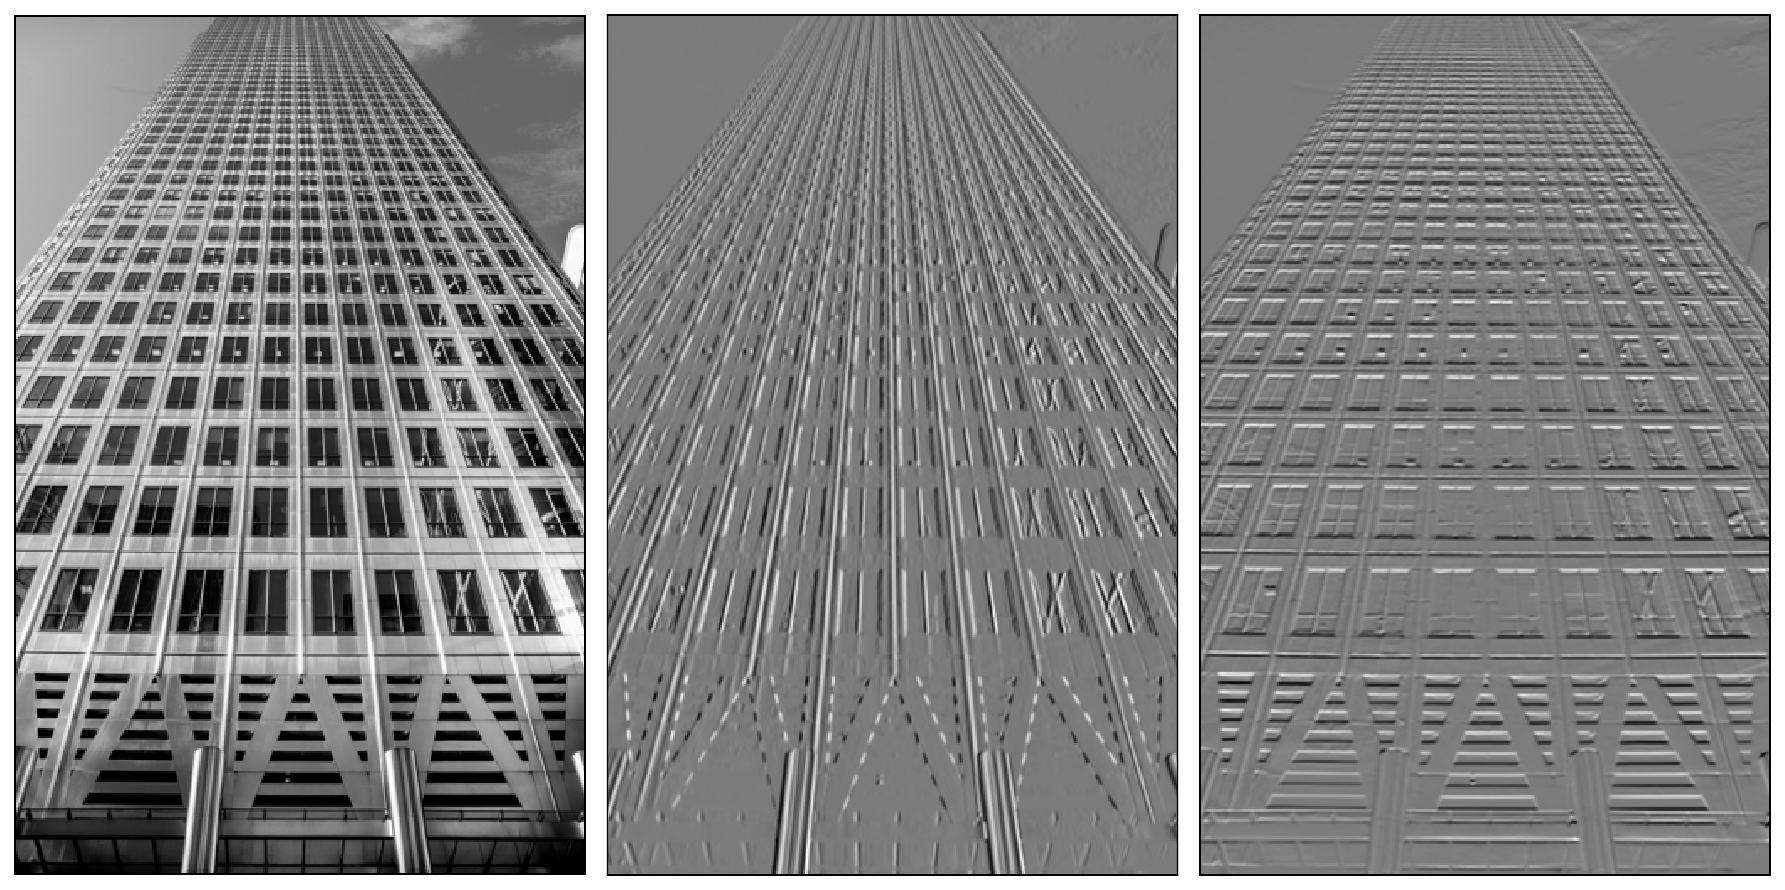
\includegraphics[width=\linewidth]{images/derivatives.pdf}
    \caption[Image derivatives]{Image derivatives. From left to right, the images represent the original image, its derivative with respect to $x$ (horizontal direction) and its derivative with respect to $y$ (vertical direction). In each of the derivative images, only the edges that are perpendicular to the direction of differentiation are visible, as expected. Source: Urban100~\cite{Huang2015}.}
    \label{fig:derivatives}
\end{figure}

Suppose we have now chosen the estimates $\frac{\partial}{\partial x}f$ and $\frac{\partial}{\partial x}f$.
Analogously to the common function, we define the image gradient (more accurately -- its estimate) as:
\begin{equation}
    \nabla f = \left( \frac{\partial}{\partial x}f, \frac{\partial}{\partial y}f \right)
\end{equation}
Thus, $\nabla f$ constitutes a particular kind of vector field (defined in Section~\ref{sss:vector_field}) known as a \textit{gradient vector field}.
Such a vector field is visualized in Figure~\ref{fig:climate_gradient} on real mean temperature data from ReKIS.
The image gradient, same as the conventional gradient, points to the direction of the biggest increase.

It is worth mentioning that the gradient usually does not point exactly to a single pixel; instead, it typically points between two pixels.
In the literature, the magnitude of this field (Equation~\eqref{e:gradient_magnitude}) is often referred to as the image gradient; nevertheless, we will treat these as distinct concepts.
In this work, we will abbreviate the approximation of the derivative of $f$ with respect to $x$ or $y$, computed from the values of the grid sampling $I$, by $\frac{\partial}{\partial x}I$ and $\frac{\partial}{\partial y}I$, respectively.
In the same manner, we will treat the estimate of the gradient of $f$ and denote it as $\nabla I$.

\begin{figure}
    \centering
    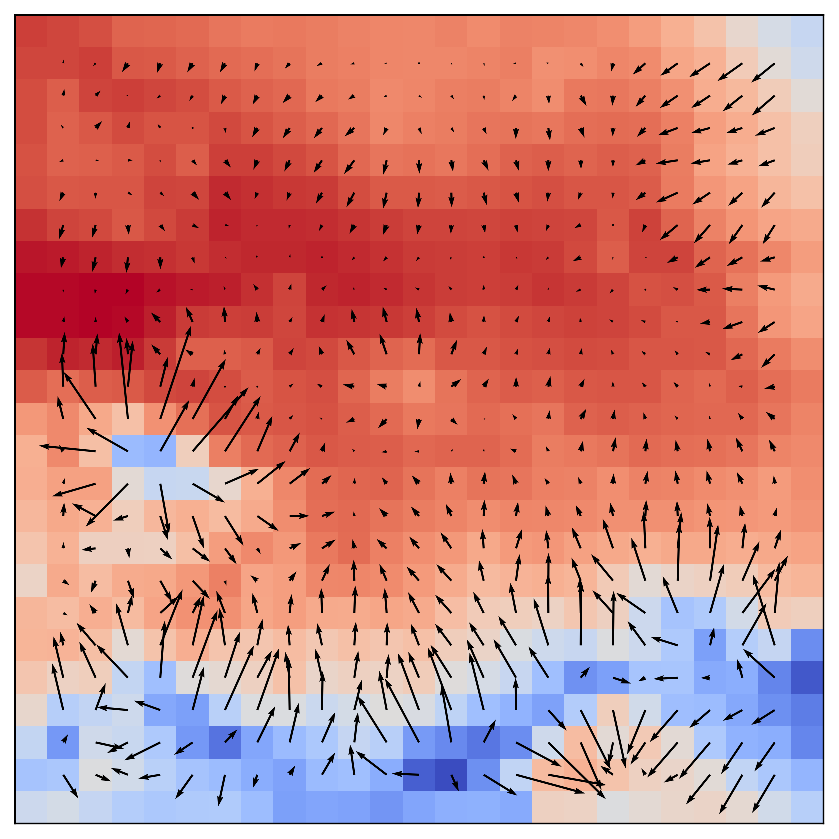
\includegraphics[width=0.5\linewidth]{images/climate_gradient.pdf}
    \caption[Image gradient]{Image gradient. Upscaled mean temperature data from ReKIS on 2000-02-01 is shown, with its gradient on top of that. As with a conventional gradient, the image gradient indicates the direction of the greatest increase in intensity.}
    \label{fig:climate_gradient}
\end{figure}

\begin{equation}
    M = \sqrt{\left( \frac{\partial}{\partial x}f\right)^2 + \left(\frac{\partial}{\partial y}f \right)^2 }
    \label{e:gradient_magnitude}
\end{equation}

\subsubsection{Vector field}
\label{sss:vector_field}

The general vector field is defined by Galbis and Maestre~\cite{Galbis2012} as a mapping that takes $n$-dimensional vectors into other $n$-dimensional vectors (Equation~\eqref{e:vector_field}).
\begin{equation}
    \mathbf{F}: U \subset \mathbb{R}^n \to \mathbb{R}^n
    \label{e:vector_field}
\end{equation}
In this work, only 2D vector fields will be used.
A vector field $\mathbf{F}$ can be represented by plotting the vectors $\mathbf{F}(\mathbf{x})$ on a grid, with each vector anchored at the point $\mathbf{x}$ (Figure~\ref{fig:climate_gradient}).
For a differentiable function $f\colon\mathbb{R}^n \to \mathbb{R}$, the mapping $\nabla f\colon\mathbb{R}^n\to\mathbb{R}^n$ defined as $\nabla f(\mathbf{x}) = \left( \frac{\partial}{\partial x_1}f(\mathbf{x}), \dots, \frac{\partial}{\partial x_n}f(\mathbf{x}) \right)$, referred to as the gradient, is a special type of vector field. 
The gradient vector field indicates, at every point in the domain of $f$, the direction of steepest increase.

\begin{figure}
    \centering
    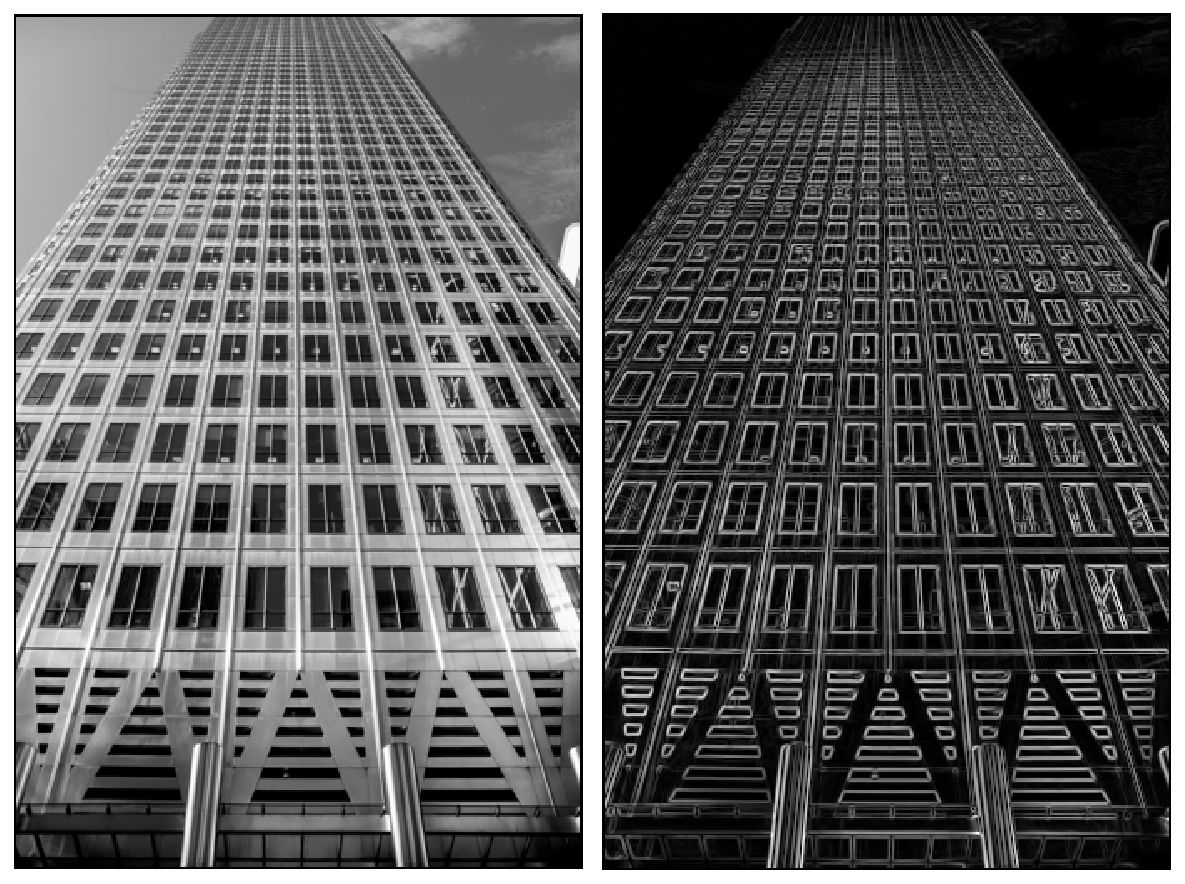
\includegraphics[width=0.66\linewidth]{images/gradient_magnitude.pdf}
    \caption[Image gradient magnitude]{Image gradient magnitude. From the derivatives in Figure~\ref{fig:derivatives} of the original image (left), image gradient magnitude (right) was calculated using Equation~\eqref{e:gradient_magnitude}. As expected, the gradient magnitude is the highest on the edges of the image and is almost zero on the same intensity regions. Source: Urban100~\cite{Huang2015}.}
    \label{fig:placeholder}
\end{figure}

\subsubsection{Dilated derivative}
\label{ss:dilated_sr_derivative}

The purpose of introducing the dilated derivative is its consistency throughout the downscaling process, which will be derived here.
Suppose we are given a high-resolution image $I^\text{HR}$, and we apply a resampling procedure -- implemented as a convolution with a kernel -- to decrease its resolution by a factor of $s$ (such as the average pooling).
For the sake of clarity, we define the downsampling operator on 2D images.

\begin{definition}[Downsampling operator]
Let $I \in \mathbb{R}^{m,n}$, $m,n\in\mathbb{N}$ be a real matrix.
For any $s \in \mathbb{N}$ such that $s \le \min(m,n)$, we define the downsampling operator $\downarrow_s$, which decreases the resolution of $I$ by a factor of $s$, as:
$$(I{\downarrow_s})[i,j] = I[is, js].$$
The output $I{\downarrow_s}$ is of dimensions $\lfloor\frac{m}{s}\rfloor \times \lfloor\frac{n}{s}\rfloor$.
\label{d:downsampling_operator}
\end{definition}
Using the downsampling operator defined in Definition~\ref{d:downsampling_operator}, the LR images can be obtained from HR images the following way:
\begin{equation}
I^\text{LR} = \left(I^\text{HR} \star k_R\right)\downarrow_s,     
\end{equation}
where $\star$ denotes the convolutional operator and $k_R$ denotes the resampling kernel of dimensions $s\times s$, for example, the average pooling kernel, filled with $s^{-2}$.
\begin{lemma}[Noble identity]
Let $I \in \mathbb{R}^{m_1,n_1}$, $m_1,n_1\in\mathbb{N}$ be a real matrix, $k \in \mathbb{R}^{m_2, n_2}$ be a real kernel, and $s\in \mathbb{N}$ be a downsampling factor.
Then the following equation holds true:
$$I{\downarrow_s}\star k = \left(I \star k^{(s)}\right){\downarrow_s},$$
where $k^{(s)}$ is a dilated kernel by $s$, meaning that between the elements of kernel $k$, $s-1$ zeros were added. 
This equation holds true only when both sides of the equation are well-defined.
\cite{Smith2011}
\label{l:noble_identity}
\end{lemma}
Lemma~\ref{l:noble_identity} will be particularly useful when $k$ is a derivative kernel $k_x$, such that $I \star k_x = \frac{\partial}{\partial x} I$; then:
\begin{equation}
\frac{\partial}{\partial x} I^\text{LR} = I^\text{LR} \star k_x = \left(I^\text{HR} \star k_R \right){\downarrow_s} \star k_x = \left(I^\text{HR} \star k^{(s)}_x \star k_R\right){\downarrow_s} = \partial_x^sI^\text{HR}.
\label{e:mean_sr_derivative}
\end{equation}
Thus, in this work, we will refer to $\partial_x^sI^\text{HR}$ as the dilated derivative by factor $s$ of $I^\text{HR}$ with respect to $x$.
The interpretation of Equation~\eqref{e:mean_sr_derivative} is that a derivative in a particular direction of a LR image is the same as the derivative in the distance of the downsampling factor of the HR image convolved with the resampling kernel and downsampled.
This allows us to enforce this relationship when downscaling between LR input and SR model output.
Furthermore, this approach is valid when applied to the gradient vector field of $I^\text{LR}$:
\begin{equation}
\begin{aligned}
    \nabla I^\text{LR} &= \left(\frac{\partial}{\partial x} I^\text{LR}, \frac{\partial}{\partial y} I^\text{LR}\right) \\
    &= \left(\partial_x^sI^\text{HR}, \partial_y^sI^\text{HR}\right).
\end{aligned}
\end{equation}

\section{Constraints}
\label{s:physical_constraints}

Some previous studies overlook that the variable being downscaled represents a physical quantity and therefore must comply with the underlying physical laws~\cite{Beucler2021}. 
The main objective, minimizing a standard pixel-wise metric (e.g., MSE, RMSE, MAE), becomes an obstacle for the model to learn physical relations, which instead produces physically inconsistent outputs only to avoid penalty~\cite{Beucler2021}. 
Therefore, if we want to improve physical consistency, we need either to penalize the physical violations or completely forbid such behavior.
Both of these strategies can be viewed as \textit{constraints}, and frameworks for their implementation have been presented by Harder et al.~\cite{Harder2023} and Beucler et al.~\cite{Beucler2021}.
In both of these works, these techniques not only lead to physically (more) consistent outputs, but the incorporation of appropriate physical constraints has exerted a demonstrably positive effect on model accuracy.

Neural networks perform mapping from the input space to the output space.
The purpose of all machine learning models is for the output to be as close to the correct solution as possible.
In the case of downscaling, the output space has a significantly higher dimension than the input space.
This provides the model with an extensive space to find the correct solution.
However, this space contains subspaces that are highly improbable or entirely impossible to contain the solution.
Temperature positivity in Kelvins is a straightforward example.
Moreover, according to the manifold hypothesis, if we pick a random point in that space, we certainly would not be close to one of the solutions, which leads us to the conclusion that the solutions are not uniformly distributed throughout the output space~\cite{Goodfellow2016}.
In conclusion, the practice of assigning a penalty to a model when its output far from our prior knowledge is known as \textit{soft-constraining}, while restricting the set of possible outputs to a particular subspace is known as \textit{hard-constraining}.

\subsection{Definition of constraints}
\label{ss:constraining}
Let $\mathbf{f}\colon \mathbb{R}^n \to \mathbb{R}^m$ be a neural network performing downscaling.
Furthermore, let $(g,h), g\colon\mathbb{R}^n \to \mathbb{R}^k, h\colon \mathbb{R}^m \to \mathbb{R}^k$ be a pair of arbitrary functions.
In these functions, it is possible to specify the constraining logic.
Then, the violation of a particular constraint is for the input LR image $I^{\text{LR}} \in \mathbb{R}^n$ and the output SR image $\mathbf{f}\left(I^{\text{LR}}\right) = I^{\text{SR}} \in \mathbb{R}^m$:
\begin{equation}
    \mathcal{L}_c = l\left(g\left(I^{\text{LR}}\right), h\left(I^{\text{SR}}\right)\right),
    \label{e:constraint}
\end{equation}
where $l$ is an evaluation metric (e.g. MAE). 

Additional definitions of constraining exist (Harder et al.~\cite{Harder2023}, Beucler et al.~\cite{Beucler2021}), but they are overly restrictive, primarily because they also prescribe a specific implementation framework.
Although those definitions are not equivalent, both agree that a constraint is a relationship between model input and output, excluding the target.

\subsection{Soft constraints}
\label{ss:soft}

Soft constraints do not directly restrict the output space.
Instead, they introduce a penalty if the output is far from our prior knowledge.
This approach is equivalent to minimizing the constraint violation $\mathcal{L}_c$ in Equation~\eqref{e:constraint}.
Training a model is minimizing its loss function; therefore, it is straightforward that soft constraints will be implemented as the loss function, representing the constraint violation itself.
Typically, $\mathcal{L}_c$ does not constitute the entire loss function; rather, it is used in conjunction with a conventional pixel-wise evaluation metric $\mathcal{L}_p$. 
Accordingly, the overall loss function $\mathcal{L}$ for a soft-constrained model is:
\begin{equation}
    \mathcal{L} = (1 - \alpha) \mathcal{L}_p + \alpha \mathcal{L}_c,
    \label{e:soft_constraint}
\end{equation}
where $\alpha \in [0, 1]$ controls the intensity of the constraint.
Every constraint matching the form in Equation~\eqref{e:constraint} can be implemented as a soft constraint in this manner.

Various works include a physically inspired modification of the loss function~\cite{Lu2019, Ge2023, Xiong2025}.
However, most of them are only loss functions -- quantifying the difference between model output (SR image) and the HR target image.
We gathered several of these methods that depend on image derivatives or gradients
and adapted them using the principle of derivative conservation under downscaling (Section~\ref{ss:dilated_sr_derivative}), enabling their use as soft constraints.

\subsubsection{Conservation law}
\label{sss:soft_conservation}

Harder et al.~\cite{Harder2023} used the mass conservation law in downscaling the column integrated water content. 
The conservation law implies that, during the downscaling process, mass or energy can neither be lost nor generated.
Thus, the goal of a soft constraint of the conservation law is to minimize the difference between the LR pixel value and the mean integrated water content of the corresponding SR pixels.
One of the experiments in~\cite{Harder2023} was to preserve column-integrated moist static energy through downscaling the same quantity along with water content and water vapor.
From these quantities, the mean temperature was calculated.
Another experiments from~\cite{Harder2023} were to apply the conservation law purely to the mean temperature, which does not have a physical background.
However, in one experiment employing this configuration, an improvement was observed relative to the baseline model.
In this work, we will focus solely on the mean temperature; therefore, the conservation law in this work will be used in a similar vein as in~\cite{Harder2023}.

Suppose that we have a LR image $I^\text{LR} \in \mathbb{R}^{n,n}$ and its $i$-th pixel $I^\text{LR}_i$.
Let $\left\{I^\text{SR}_{i, j} \mid j=1,\dots,s^2\right\}$ be the corresponding set of pixels downscaled from $I^\text{LR}_i$ by a scale factor $s$.
Then, the conservation law is defined by the equation:
\begin{equation}
    I^\text{LR}_i = \frac{1}{s^2}\sum_{j=1}^{s^2}I^\text{SR}_{i, j}
    \label{e:conservation}
\end{equation}
for each $i = 1, \dots, n$. 
In summary, the conservation law entails preserving a physical quantity, such as mass or energy, so that the mean value of the downscaled pixels remains equal to that of the corresponding original LR pixel.
Naturally, in soft constraining, the error between the two sides of Equation~\eqref{e:conservation} will be minimized.
We note that the right side of Equation~\eqref{e:conservation} is equivalent to average pooling with a kernel of size $s \times s$.
Therefore, we can denote the later average pooling output as $\bar{I}^\text{SR}$. 
The constraint violation is then:
\begin{equation}
    \mathcal{L}_c = l\left(I^\text{LR}_i, \bar{I}^\text{SR}\right),
\end{equation}
for an evaluation metric $l$ (MAE and MSE will be implemented and experimented with).

\subsubsection{Simple derivative constraint}

The derivative constraint, as its name suggests, is a very straightforward continuation of Section~\ref{ss:dilated_sr_derivative}.
The constraint builds upon the fact that both $I^\text{LR}$ partial derivatives $\frac{\partial}{\partial x}I^\text{LR}$ and $\frac{\partial}{\partial y}I^\text{LR}$ are the same as the dilated derivatives $\partial_x^sI^\text{HR}$ and $\partial_y^sI^\text{HR}$ of $I^\text{HR}$.
This suggests the penalization of this difference in the case of  $I^\text{SR}$.
So the constraint violation is:
\begin{equation}
    \mathcal{L}_c = l\left(\frac{\partial}{\partial x} I^\text{LR}, \partial^s_x I^\text{SR}\right) + l\left(\frac{\partial}{\partial y} I^\text{LR}, \partial^s_y I^\text{SR}\right),
\end{equation}
where $l$ is an evaluation metric; in this work, MAE and MSE will be used.
To obtain the derivatives with respect to $x$ and $y$, the convolution of the image with simple (Equation~\eqref{e:simple_derivative_kernels}) kernels will be used.

\subsubsection{Sobel gradient magnitude constraint}

Lu and Chen~\cite{Lu2019} improved an U-Net architecture for downscaling natural images by using an additional loss term -- gradient magnitude difference.
For pairs of $I^\text{SR}$ and $I^\text{HR}$, they calculated the image derivatives $\frac{\partial}{\partial x} I^\text{SR}$, $\frac{\partial}{\partial y} I^\text{SR}$, $\frac{\partial}{\partial x} I^\text{HR}$, and $\frac{\partial}{\partial y} I^\text{HR}$ using Sobel kernels.
Then, for both $I^\text{SR}$ and $I^\text{HR}$, they obtained gradient magnitudes $M^\text{SR}$ and $M^\text{HR}$ from the derivatives using Equation~\eqref{e:gradient_magnitude}. 
The loss function was the MSE between $I^\text{SR}$ and $I^\text{HR}$, and the MSE between the gradient magnitudes $M^\text{SR}$ and $M^\text{HR}$.
However, this is not a constraint as defined in Section~\ref{ss:constraining} because it also depends on the HR image.
Thus, the modification of this process is required.
This is done by computing the dilated SR derivatives Section~\ref{ss:dilated_sr_derivative} using Sobel kernels with respect to $x$ and $y$, resulting in $\partial^s_x I^\text{SR}, \partial^s_y I^\text{SR}$.
Again, the magnitude of the SR gradient is computed using the Equation~\eqref{e:gradient_magnitude}; however, in this case, the dilated SR derivatives are used:
\begin{equation}
    \bar{M}^{SR} = \sqrt{\left(\partial^s_x I^\text{SR}\right)^2 + \left(\partial^s_y I^\text{SR}\right)^2}.
\end{equation}
Therefore, the final soft constraining loss will be:
\begin{equation}
    \mathcal{L}_c = l\left(\bar{M}^\text{SR}, M^\text{LR}\right) 
\end{equation}
for a voluntary evaluation metric $l$.

\subsubsection{Temperature field continuity}

Xiong~\cite{Xiong2025} used a modified loss function for spatiotemporal downscaling of temperature near the Yangtze River.
In the work, the term temperature field continuity was used as the square of the difference between neighboring pixels in the horizontal and vertical directions.
This is equivalent to the square of a derivative computed by a trivial kernel (Equation~\eqref{e:trivial_derivative_kernels}).
Therefore, the used loss function can be described as:
\begin{equation}
    \begin{aligned}
        E_c &= \biggl|\sum\left(\frac{\partial}{\partial x} I^\text{SR}\right)^2 + \sum\left(\frac{\partial}{\partial y}I^\text{SR}\right)^2 \\
        &- \sum\left(\frac{\partial}{\partial x}I^\text{HR}\right)^2 - \sum\left(\frac{\partial}{\partial y}I^\text{HR}\right)^2\biggr|.
    \end{aligned}
    \label{e:xiong_continuity}
\end{equation}
However, Equation~\eqref{e:xiong_continuity} does not act as a constraint, since it also relies on HR images.
We adjust the loss function by removing $I^\text{HR}$, incorporating $I^\text{LR}$, and applying the dilated derivatives of $I^\text{SR}$ described in Section~\ref{ss:dilated_sr_derivative}. 
In addition, $E_c$ may grow excessively for large images or batch sizes; thus, we take the mean over pixels.
Equations~\eqref{e:continuity} show the modifications made to stabilize the loss function values and to comply with the soft constraining definition in the absolute, resp. square version.

\begin{equation}
    \begin{aligned}
    \mathcal{L}_c^\text{A} &= \frac{1}{N} \biggl|\sum\left|\partial^s_xI^\text{SR}\right| + \sum\left|\partial^s_yI^\text{SR}\right| \\
    &- \sum\left|\frac{\partial}{\partial x} I^\text{LR}\right| - \sum\left|\frac{\partial}{\partial y}I^\text{LR}\right|\biggr| \\
    \mathcal{L}_c^\text{S} &= \frac{1}{N}\biggl|\sum\left(\partial^s_x I^\text{SR}\right)^2 + \sum\left(\partial^s_y I^\text{SR}\right)^2 \\
    &- \sum\left(\frac{\partial}{\partial x}I^\text{LR}\right)^2 - \sum\left(\frac{\partial}{\partial y}I^\text{LR}\right)^2\biggr|
    \end{aligned}
    \label{e:continuity}
\end{equation}

\subsubsection{Gradient direction constraint}

Xiong~\cite{Xiong2025} inspired us to focus on the gradient directions, not only the magnitudes.
The above approaches depend on the derivatives or the magnitude of the gradient, not its orientation.
Xiong~\cite{Xiong2025} applied the \textit{atan2} function to pairs of horizontally and vertically adjacent pixels, summed these results, and then computed the difference between the SR output and the HR target, as shown in Equation~\eqref{e:xiong_dir_continuity}.
These values, however, did not correspond to any particular angles; they only captured global characteristics of the field.
\begin{equation}
    \begin{aligned}
        \mathcal{L}_d = \biggl| 
        \sum_{i = 1}^M\sum_{j = 1}^{N-1} \text{atan2}\left(I^\text{SR}_{i,j}, I^\text{SR}_{i,j + 1}\right) & +
        \sum_{i = 1}^{M - 1}\sum_{j = 1}^{N} \text{atan2}\left(I^\text{SR}_{i,j}, I^\text{SR}_{i+1,j}\right) \\ -
        \sum_{i = 1}^M\sum_{j = 1}^{N-1} \text{atan2}\left(I^\text{HR}_{i,j}, I^\text{HR}_{i,j + 1}\right) & -
        \sum_{i = 1}^{M - 1}\sum_{j = 1}^{N} \text{atan2}\left(I^\text{HR}_{i,j}, I^\text{HR}_{i+1,j}\right)
        \biggr|
    \end{aligned}
    \label{e:xiong_dir_continuity}
\end{equation}
However, the Equation~\eqref{e:xiong_dir_continuity} does not comply with the constraining setup.
It uses the HR target; instead, we will define it for LR input and dilated SR derivatives.
Furthermore, we will modify the function by incorporating local elements that are interpretable.
The key idea is to compare the orientations of the LR gradient and the dilated SR gradient vectors in each point of the image.
We will employ the cosine similarity function for this purpose, defined as:
\begin{equation}
    \text{cos\_sim}(u, v) = \frac{u \cdot v}{\|u\|\cdot\|v\|},
    \label{e:cos_sim}
\end{equation}
where $u,v$ are two dimensional vectors.
This function's range is $[-1, 1]$, when the direction of $u$ and $v$ is the same, resp. is perpendicular, resp. is exactly the opposite, their cosine similarity is equal to $1$, resp. $0$, resp. $-1$.
Therefore, we first calculate the dilated SR derivatives $\partial_x^s I^\text{SR}$, $\partial_y^s I^\text{SR}$ of the SR image with respect to $x$ and $y$.
If the $\partial_x^s I^\text{SR}$, $\partial_y^s I^\text{SR}$ are not the same shapes as a result of the derivative kernel choice, they need to be trimmed.
Then we can calculate the angle similarity matrix S as:
\begin{equation}
    \text{S} = 
    \text{cos\_sim}\left(\left(\partial^s_x I^\text{SR}, \partial^s_y I^\text{SR} \right), \left(\frac{\partial}{\partial x} I^\text{LR}, \frac{\partial}{\partial y} I^\text{LR}\right)\right),
\end{equation}
where the cos\_sim function is applied element-wise to matching indices in the matrices, resulting in a matrix.
Furthermore, we will scale the errors by the magnitude of the LR gradient (Equation~\eqref{e:magnitude}) in the corresponding point because we do not want to punish large angle differences in areas where the gradient magnitude is almost zero.
\begin{equation}
    \text{M} = \sqrt{\left(\frac{\partial}{\partial x} I^\text{LR}\right)^2 + \left(\frac{\partial}{\partial y} I^\text{LR}\right)^2}
\label{e:magnitude}
\end{equation}
Therefore, the final constraint violation will be:
\begin{equation}
    \begin{aligned}
        \mathcal{L}_c^\text{A} &= \frac{1}{mn}\sum_{i = 1}^m\sum_{j = 1}^n(1-S_{i,j})M_{i,j}, \\
        \mathcal{L}_c^\text{S} &= \frac{1}{mn}\sum_{i = 1}^m\sum_{j = 1}^n\left((1-S_{i,j})M_{i,j}\right)^2.
    \end{aligned}
\end{equation}

To obtain the derivatives with respect to $x$ and $y$, the convolution of the image with simple (Equation~\eqref{e:simple_derivative_kernels}), resp. Sobel (Equation~\eqref{e:Sobel_kernels}) kernels will be used; in that case, we will refer to this constraint as simple, resp. Sobel gradient direction constraint.

\subsubsection{G-Loss}

Ge and Dou~\cite{Ge2023} introduced a G-Loss loss function for downscaling natural images.
It belongs to other derivative-difference-based loss functions, as mentioned above.
However, its uniqueness is hidden in the usage of the derivatives in a distance $s$ in the HR image for downscaling with a downscaling factor $s$ and the derivatives being with respect to all 8 directions.
The loss is applied on HR and SR images. 
It consists of pixel-wise loss and a derivative-difference-inspired approach. 

When the downscaling is done with a scale factor of 1, only the derivatives are compared by L1-loss in addition to the direct L1-loss between the HR and SR images, as shown in Figure~\ref{fig:gloss}. 
However, when the scale factor is larger, average or max pooling can be applied to both HR and SR images, and afterward, the result is convolved with the derivative kernels.
The extracted patches from the LR and HR images are evaluated using an L1 loss between them.

Nevertheless, the results in~\cite{Ge2023} were the best when splitting (pixel shuffle) layers were used instead of average or max pooling layers.
The interpretation of the latter approach is that the derivative kernels are applied to the neighboring pixels in the split patches; however, those are in a distance of the scale factor $s$ in the original image, as visible in Figure~\ref{fig:mean_sr_gradient}.
Moreover, the process of convolving the split patches with derivative kernels is equivalent to performing a dilated convolution on the original images.
Therefore, if we pick one particular derivative kernel, convolve the split patches by it, and calculate the mean across the resulting patches, we obtain the dilated derivative. 
Thus, to convert this loss function -- more precisely, the part containing the splitting and derivative computation -- into a soft constraint, we use the dilated derivatives of $I^\text{SR}$ and compare them with the derivatives of $I^\text{LR}$.

\begin{figure}[htbp]
    \centering
    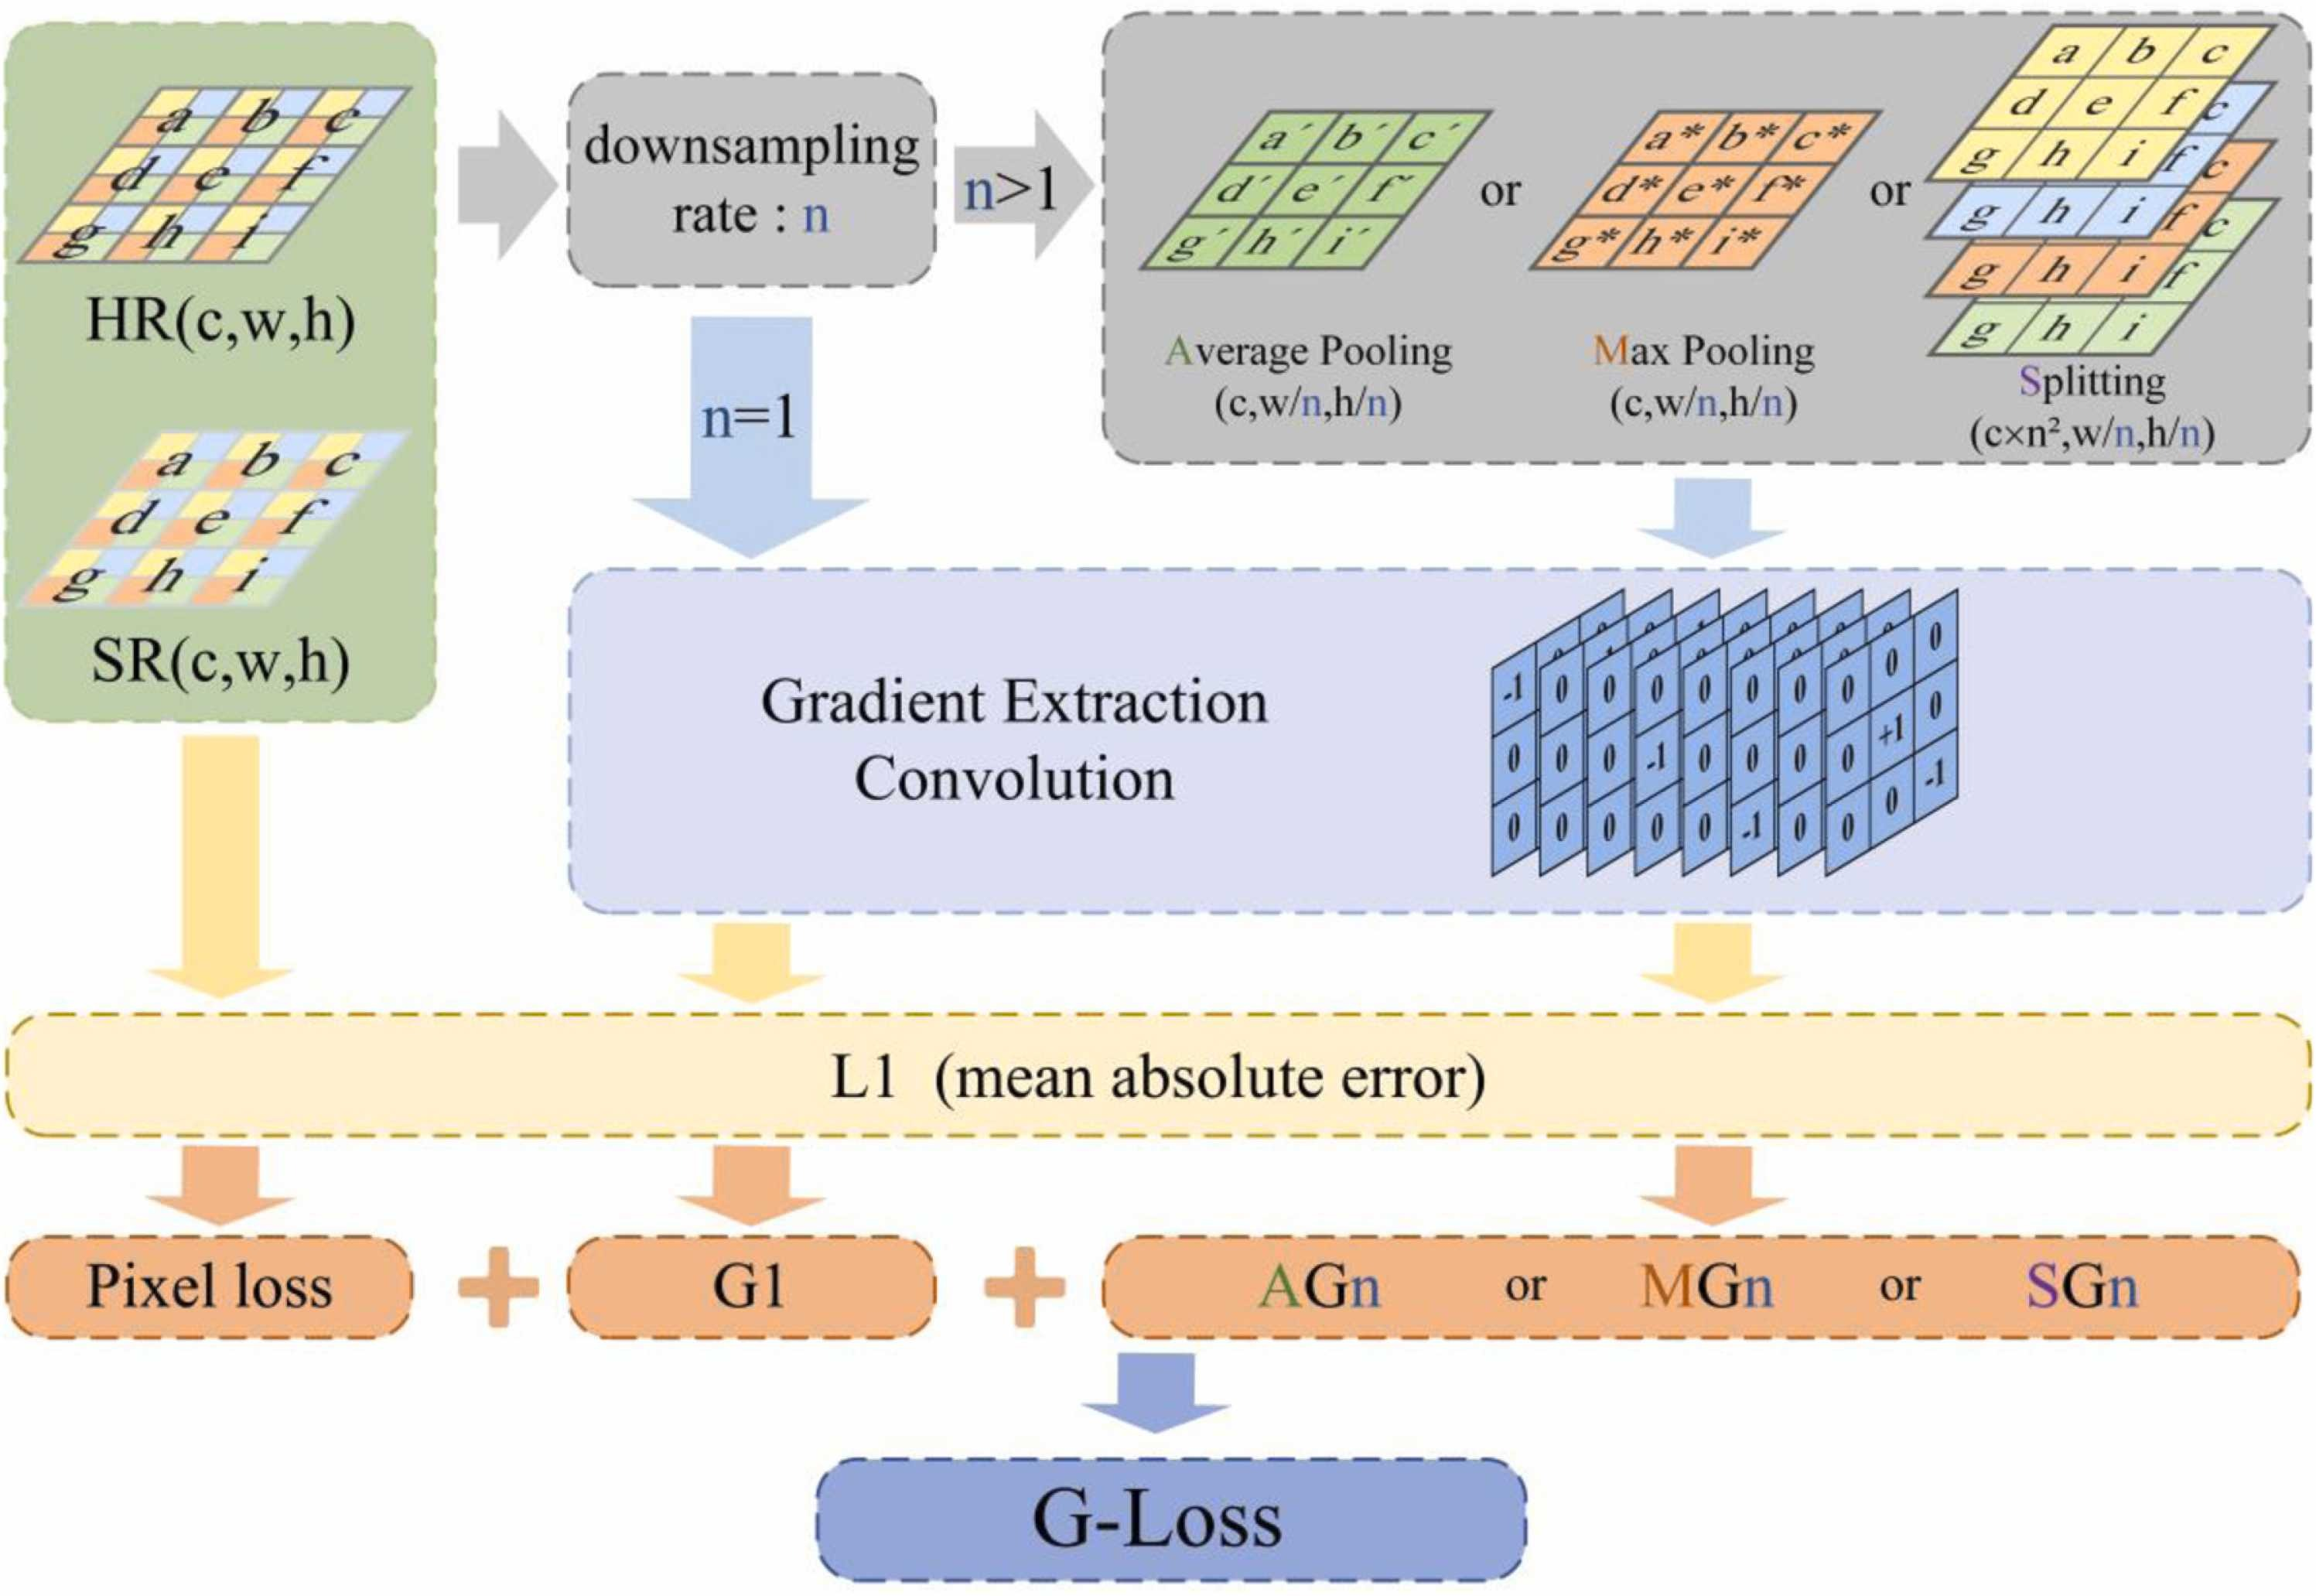
\includegraphics[width=0.8\linewidth]{images/gloss.jpg}
    \caption[G-Loss]{G-Loss. Source: Ge and Dou~\cite{Ge2023}.}
    \label{fig:gloss}
\end{figure}

The constraint violation is dependent on the derivatives in all eight directions.
They will be calculated using the kernels in Equation~\eqref{e:direction_kernels}.
\begin{equation}
    \begin{aligned}
        K = \Biggl\{ 
            &\begin{bmatrix} -1 & 0 & 0 \\ 0 & 1 & 0 \\ 0 & 0 & 0 \end{bmatrix},
            \begin{bmatrix}  0 & -1 & 0 \\ 0 & 1 & 0 \\ 0 & 0 & 0 \end{bmatrix},
            \begin{bmatrix}  0 & 0 & -1 \\ 0 & 1 & 0 \\ 0 & 0 & 0 \end{bmatrix},
            \begin{bmatrix}  0 & 0 & 0 \\ -1 & 1 & 0 \\ 0 & 0 & 0 \end{bmatrix}, \\
            &\begin{bmatrix}  0 & 0 & 0 \\ 0 & 1 & -1 \\ 0 & 0 & 0 \end{bmatrix},
            \begin{bmatrix}  0 & 0 & 0 \\ 0 & 1 & 0 \\ -1 & 0 & 0 \end{bmatrix},
            \begin{bmatrix}  0 & 0 & 0 \\ 0 & 1 & 0 \\ 0 & -1 & 0 \end{bmatrix},
            \begin{bmatrix}  0 & 0 & 0 \\ 0 & 1 & 0 \\ 0 & 0 & -1 \end{bmatrix}
            \Biggr\}
    \end{aligned}
    \label{e:direction_kernels}
\end{equation}
Therefore, the constraint violation will be:
\begin{equation}
    \mathcal{L}_c = l\left( \left( \partial_{K_1}^s I^\text{SR}, \dots, \partial_{K_8}^s I^\text{SR} \right), \left( \frac{\partial}{\partial K_1} I^\text{LR}, \dots, \frac{\partial}{\partial K_8} I^\text{LR}\right) \right)
\end{equation}
for $l$ being an evaluation metric, in this work MAE and MSE are used.

\begin{landscape}
    \begin{figure}[htbp]
        \centering
        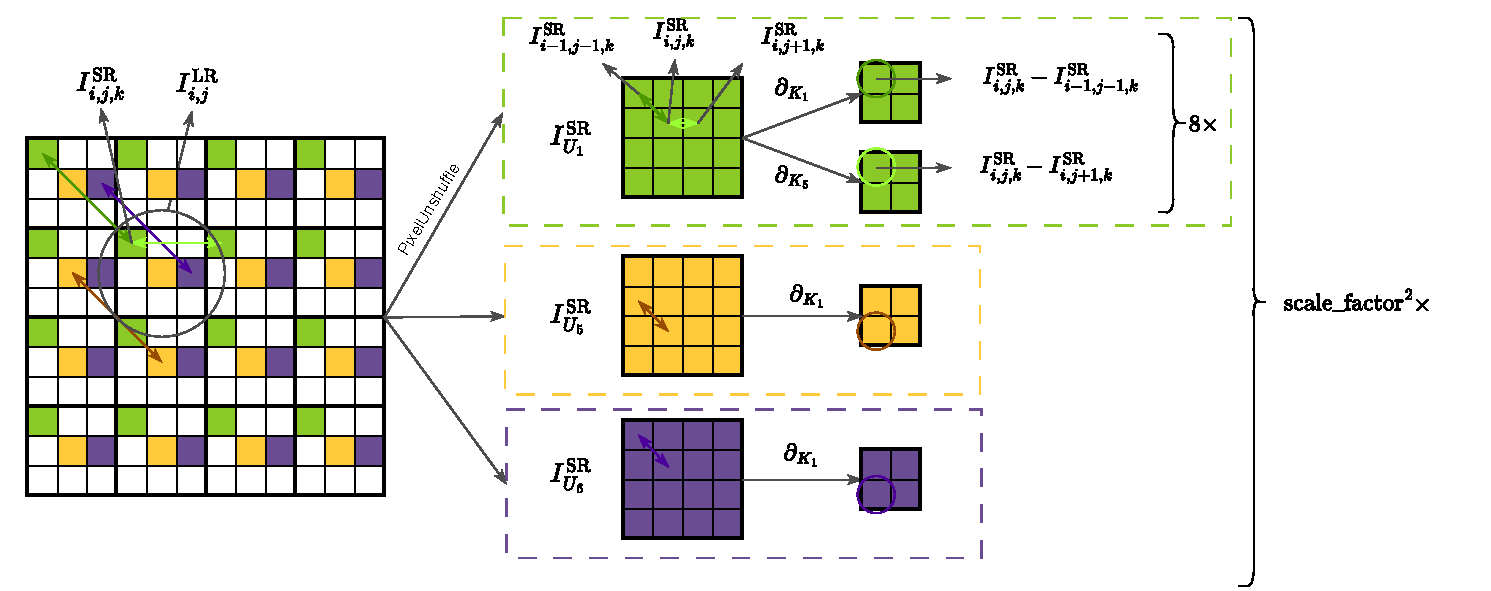
\includegraphics[width=\linewidth]{images/gloss.pdf}
        \caption[G-Loss patch derivatives]{
        G-Loss patch derivatives. 
        Downscaling factor $s = 3$ was used as example. 
        The indexation of the image is different than from the rest of the work.
        Here, the $I^\text{LR}_{i,j}$ corresponds to the pixel in the LR image in the $i$-th row and $j$-th column.
        This pixel is then downscaled producing pixels $\left\{I_{i,j,k}^\text{SR} \mid k \in \{1, 2, \dots s^2\}\right\}$.
        The derivative kernels are each of size $3\times3$ and are shown in Equation~\eqref{e:direction_kernels}. 
        No padding is added in convolution with derivative kernels.
        It is evident, that convolving the derivative kernels on the unshuffled patches is equivalent to convolving them with dilation.
        Furthermore, computing the mean over the unshuffled derivative patches (on the right side of the visualization) in direction $K_d$ produces the dilated derivative (Section~\ref{ss:dilated_sr_derivative}) in the direction $K_d$.
        For example, in the direction $K_1$ there are $s^2$ derivative patches (3 of them are shown on the right side).
        The element-wise mean of all the $s^2$ patches is equal to the dilated derivative in the direction $K_1$.
        }
        \label{fig:mean_sr_gradient}
    \end{figure}
\end{landscape}

\subsection{Hard constraints}

Hard constraints force the model to yield outputs that are consistent with the defined constraints.
In contrast to soft constraints (Section~\ref{ss:soft}), minimizing the constraint violation is insufficient in this case; the goal is to completely eliminate any constraint violation:
\begin{equation}
    \mathcal{L}_c = l\left(g\left(I^{\text{LR}}\right), h\left(I^{\text{SR}}\right)\right) = 0.
    \label{e:hard}
\end{equation}

To achieve the Equation~\eqref{e:hard}, model architecture changes are needed to guaranty the output's compliance with restrictions.
This change is implemented by adding one or more constraint layers.
Not every constraint in the form of Equation~\eqref{e:constraint} can be implemented straightforwardly as a hard constraint.

In a similar vein as soft constraint, Harder et al.~\cite{Harder2023} proposed the enforcement of the conservation law in the form of a hard constraint.
For the purpose of atmospheric gas concentration downscaling, Geiss et al.~\cite{Geiss2022} used a final constraining layer after SRCNN. 
However, this was not enough to improve the accuracy of the baseline model, except for ozone downscaling. 

\subsubsection{Non-negativity enforcing hard constraint layer}

Many variables cannot be negative, e.g., age, length, or climate related temperature in Kelvins.
Hence, it makes sense to have a non-negativity enforcing layer in some models.
To match the constraining setup (Section~\ref{ss:constraining}) we set 
\begin{equation}
\begin{aligned}
    \left(\forall I^{\text{LR}} \right) g\left(I^{\text{LR}}\right) = 0
    \ &\wedge \ 
h\left(I^{\text{SR}}\right) = \min_{i,j}\left(0, I^\text{SR}_{i,j}\right),
\end{aligned}
\end{equation}
therefore, the 
\begin{equation}
\mathcal{L}_s = g\left(I^{\text{LR}}\right) - h\left(I^{\text{SR}}\right)    
\end{equation}
will be zero if and only if all pixels in $I^\text{SR}$ are non-negative.
This trivial case could be solved by adding ReLU as the output layer of our network.

\subsubsection{General hard constraint layers}

For arbitrary constraints in the form as in our constraint setup (Section~\ref{ss:constraining}), there is no known general procedure to implement hard constraints.
We will need a more specific setup to automatically implement hard constraints.
\newpage
Harder et al. \cite{Harder2023} provided a generalization for constraining in the case of downscaling.
Suppose that we have an input LR image $I^{\text{LR}} \in \mathbb{R}^n$ and an output SR image $I^{\text{SR}} \in \mathbb{R}^m$.
Now $(S_j)_{j = 1, \dots, n}$ is a partition of $\{1, \dots, m\}$ into $n$ subsets, $g_{ij} : \mathcal{D} \subset \mathbb{R} \to \mathbb{R}, i \in S_j$ is an invertible function, and $h_j:\mathbb{R}^n \to \mathbb{R}$ is an arbitrary function.
The set of constraints is given by:
\begin{equation}
    \sum_{i\in S_j}g_{ij}\left(I^\text{SR}_i\right) = h_j\left(I^{\text{LR}}\right),
    \label{e:harder_constraint}
\end{equation}
for each $j = 1, \dots, n$.
Note that in downscaling with a scale factor of $s$, all the $S_j$ have a size of $s^2$.
Not every soft constraint mentioned in this work can be converted into a hard constraint.
Mainly, the approaches using the dilated derivatives cannot be expressed in the form of Equation~\eqref{e:harder_constraint} because the dilated derivative does not operate solely on the $s\times s$ patches, but also uses information from the neighboring patches.

Suppose that we have our general constraint in the form of Equation~\eqref{e:harder_constraint}.
Harder et al.~\cite{Harder2023} implemented three different approaches to a hard constraint layer -- additive, multiplicative, and soft-max layers.
These are defined by their output:
\begin{equation}
\begin{aligned}
    y_i^\text{AddCL} &= g_{ij}^{-1}\left( \tilde{y}_i + \frac{1}{s^2} h_j\left(I^{\text{LR}}\right) - \frac{1}{s^2} \sum_{k\in S_j}\tilde{y}_k \right), \\
    y_i^\text{MultCL} &= g_{ij}^{-1}\left( \tilde{y}_i \cdot \frac{h_j\left(I^{\text{LR}}\right)}{\sum_{k\in S_j}\tilde{y}_k }\right), \\
    y_i^\text{SmCL} &= g_{ij}^{-1}\left( \exp\left(\tilde{y}_i\right) \cdot \frac{h_j\left(I^{\text{LR}}\right)}{\sum_{k\in S_j}\exp\left(\tilde{y}_i\right) }\right), \\
\end{aligned}
\label{e:hard_constraint_layers}
\end{equation}
for $j = 1, \dots, n$, where the output from the unconstrained model is labeled as $\tilde{y}$.

\subsubsection{Conservation law}

Analogously to its soft-constraint counterpart (Section~\ref{sss:soft_conservation}), the enforced relation is that each LR pixel value is conserved and corresponds to the mean of the pixels generated from that specific pixel.
Formally, the enforced relation is:
\begin{equation}
    I^\text{LR}_{j} = \frac{1}{s^2} \sum_{i \in S_j}I^\text{SR}_{i}.
\end{equation}

The conservation law can be implemented as a hard constraint because it complies with Equation~\eqref{e:harder_constraint}.
This can be implemented with a standard deep learning model, augmented by an additional output layer -- a \textit{constraining layer} -- that modifies the model output in such a manner that the output LR pixel is equal to the mean of its corresponding downscaled SR pixels.
For this purpose, we will use the general Equations~\eqref{e:hard_constraint_layers} of hard constraint layers, with $g_{ij}$ being an identity function and $h_j(I^\text{LR}) = s^2 I^\text{LR}_j$.
The process of the additive constraint layer is depicted in Figure~\ref{fig:hard_conservation}.

\begin{figure}[htbp]
    \centering
    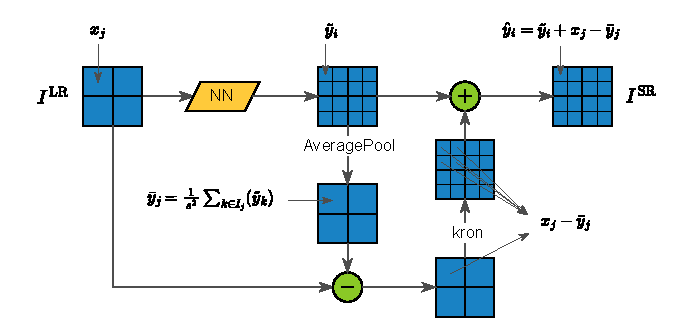
\includegraphics[width=\linewidth]{images/hard_conservation.pdf}
    \caption[Conservation law -- hard constraint]{Conservation law -- hard constraint. The operation ``kron'' denotes the Kronecker product (as defined in Section~\ref{sss:kronecker}) of the displayed matrix with an $s \times s$ matrix whose entries are all ones. Generating an output that matches the dimensions of the NN’s output.}
    \label{fig:hard_conservation}
\end{figure}

We will now prove that the implementation of the additive constraint layer (Equation~\eqref{e:hard_constraint_layers}) with the setup specified above and the implementation in Figure~\ref{fig:hard_conservation} is correct.

\begin{proof}
First, we state the output of the additive constraint layer (Equation~\eqref{e:hard_constraint_layers}) with the setup of $g_{ij}$ being an identity function and $h_j(I^\text{LR}) = s^2 I^\text{LR}_j$.
$$
I_i^\text{SR} = y_i^\text{AddCL} = \tilde{y}_i + I^\text{LR}_j - \frac{1}{s^2} \sum_{k\in S_j}\tilde{y}_k
$$
Now we calculate the means over areas $S_j$ for each $j$:
$$
\begin{aligned}
    \frac{1}{s^2} \sum_{i \in S_j} y_i^\text{AddCL} &=
    \frac{1}{s^2} \sum_{i \in S_j} \left(\tilde{y}_i + I^\text{LR}_j - \frac{1}{s^2} \sum_{k\in S_j}\tilde{y}_k \right) \\
    &= \frac{1}{s^2} \sum_{i \in S_j} \left(\tilde{y}_i \right) + I^\text{LR}_j - \frac{1}{s^2} \sum_{k\in S_j} \left(\tilde{y}_k \right) \\
    &= I_j^\text{LR}
\end{aligned}
$$
Thus, the means over areas of $S_j$ for each $j$ are equal to the corresponding input pixel $I_j^\text{LR}$.
\end{proof}

The proofs for the multiplicative and soft-max constraint layers closely follow the one given above; since the key step is merely replacing the output value, we do not present them here.

\subsubsection{Kronecker product}
\label{sss:kronecker}

The Kronecker product is a binary operation on two matrices of arbitrary sizes $A \in \mathbb{R}^{m_1, n_1}, B \in \mathbb{R}^{m_2, n_2}$, defined as:
\begin{equation}
    A \otimes B \coloneqq 
    \begin{bmatrix}
        A_{1,1} \cdot B & \cdots & A_{1, n} \cdot B \\
        \vdots & \ddots & \vdots \\ 
        A_{m, 1} \cdot B & \cdots & A_{m, n} \cdot B \\
    \end{bmatrix}.
\end{equation}
The result $A \otimes B$ is therefore the matrix $B$ multiplied by all scalars of $A$. 
For each of $m_1$ rows of $A$, the scalars will multiply $m_2$ rows of B; the same applies for columns, leading us to the dimension of the result being $(m_1 \cdot m_2) \times (n_1 \cdot n_2)$.

\subsection{Physical constraints}

There is not a distinct border between non-physical and physical constraints.
We consider any constraint that enforces physical laws, or that operates on physics-related quantities such as shape, gradients, and similar indicators, to be a physical constraint.

\section{Multivariate downscaling}

Multivariate downscaling refers to the simultaneous downscaling of several physical variables.
Furthermore, it allows for the incorporation of more complex physical relationships between the downscaled variables.
For example, Rocha et al.~\cite{Rocha2025} used up to five variables to downscale sea ice concentration.
Furthermore, Harder et al.~\cite{Harder2023} required surface temperature, liquid water, and water vapor in order to compute moist static energy, downscale the last three quantities and subsequently derive SR temperature from them.
However in this work we will focus solely on the mean temperature.

\section{Resampling}

There are several approaches for converting between HR and LR grids.
The simplest one is \textit{nearest} resampling, in which the value of a pixel at a new location is simply taken from the closest existing pixel.
A more advanced option is \textit{bilinear} interpolation, in which the value of the new pixel is obtained as a distance-weighted average of the surrounding pixels in the $2 \times 2$ neighborhood.
Both \textit{cubic} and \textit{cubic spline} methods use cubic polynomial approximations over $4 \times 4$ neighborhoods; however, cubic spline typically yields smoother transitions.
For more information about the above methods see Roszkowiak et al.~\cite{Roszkowiak2017}.
\textit{Lanczos} resampling relies on an even larger $6 \times 6$ neighborhood and evaluates the new pixel value using the $\text{sinc}$ function.
Detailed description can be found in Mazzoli~\cite{Mazzoli2026}.
When the value of a new pixel is obtained as the average over a neighborhood of arbitrary size, the procedure is referred to as \textit{average} resampling.
